\documentclass[aspectratio=169, 10pt]{beamer}

\usefonttheme{professionalfonts}
\usepackage{tikz}
\usetikzlibrary{shapes.geometric, arrows.meta, positioning, calc}
\usepackage{booktabs}
\usepackage{caption}

\usetheme{Madrid}
\usecolortheme{dolphin}

\title[RayCastED]{RayCastED: A RayCast End-to-end Detection Model for Lightweight and Boundary-Aware Nuclei Detection}
\author[Danish Dhiaurrahman Ritonga]{Danish Dhiaurrahman Ritonga}
\institute[DTETI UGM]{
  Department of Electrical Engineering and Information Technology\\
  Universitas Gadjah Mada
}
\date{2026}

\begin{document}

\begin{frame}
  \titlepage
\end{frame}


\section{Motivation}

\begin{frame}{Clinical Background: TILs Assessment}
  \begin{columns}
    \column{0.6\textwidth}
    \begin{itemize}
      \item \textbf{Tumor-infiltrating lymphocytes (TILs)} are established prognostic biomarkers in multiple cancers
      \item International TILs Working Group guidelines recommend \textbf{area-based scoring}: percentage of stromal area occupied by lymphocytes
      \item \textbf{Critical requirement}: accurate boundary delineation, not just centroid detection
    \end{itemize}

    \column{0.4\textwidth}
    \begin{alertblock}{The Challenge}
      Manual assessment is:
      \begin{itemize}
        \item Time-consuming
        \item Subject to inter-observer variability
        \item Impractical for whole-slide images
      \end{itemize}
    \end{alertblock}
  \end{columns}
\end{frame}

\begin{frame}{The Clumped Cell Problem}
  \begin{columns}
    \column{0.55\textwidth}
    \begin{itemize}
      \item Densely clustered nuclei merge in segmentation masks
      \item FCN-based models produce contiguous predictions
      \item \textbf{Result}: Systematic undercounting
      \item Existing solutions require costly post-processing
      \item NMS suppresses overlapping predictions (risky in clumped regions)
    \end{itemize}

    \column{0.45\textwidth}
    \begin{exampleblock}{Key Issues}
      \begin{enumerate}
        \item Instance separation overhead
        \item NMS-based suppression errors
        \item Deployment inaccessibility (transformers)
      \end{enumerate}
    \end{exampleblock}
  \end{columns}
\end{frame}



\begin{frame}{The Accuracy-Deployment Trade-off}
  \begin{center}
    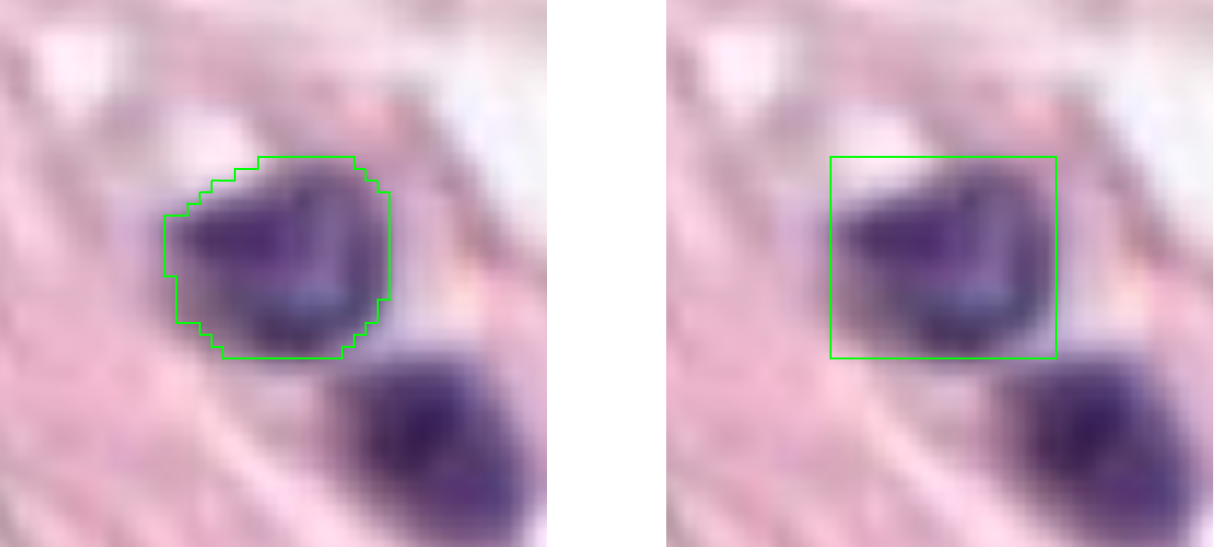
\includegraphics[width=0.45\textwidth]{fig/seg-vs-det.png}
  \end{center}

  \begin{table}
    \centering
    \small
    \begin{tabular}{lp{5cm}p{4cm}}
      \toprule
      \textbf{Approach} & \textbf{Pros} & \textbf{Cons} \\
      \midrule
      Instance Segmentation & Accurate boundaries & Computationally expensive \\
      (U-Net, Mask R-CNN) & & (unsuitable for edge) \\
      \midrule
      Transformer-based & Strong performance & Quadratic complexity \\
      (CellViT, DINO) & Good separation & (memory/compute intensive) \\
      \midrule
      Object Detection & Fast, lightweight & \textbf{No boundary geometry} \\
      (YOLO, Faster R-CNN) & Edge-deployable & (insufficient for TILs) \\
      \bottomrule
    \end{tabular}
  \end{table}

\end{frame}


\section{Star-Convex Representation}

\begin{frame}{Star-Convex Polygons for Cell Representation}
  \begin{center}
    \begin{tikzpicture}
      % Left: Pure TikZ diagram of star-convex polygon (polar coordinates)
      \begin{scope}[shift={(-4,0)}]
        % Concentric grid circles
        \foreach \r in {0.5, 1.0, 1.5, 2.0} {
          \draw[gray!30, thin] (0,0) circle (\r);
        }

        % Radial grid lines every 30 degrees
        \foreach \a in {0,30,...,330} {
          \draw[gray!30, thin] (0,0) -- (\a:2.1);
        }

        % Polar axis labels
        \draw[->, gray!60] (0,0) -- (2.3,0) node[right, font=\small] {$\theta = 0$};
        \draw[gray!60, dashed] (0,0) -- (90:2.1) node[above, font=\small] {$\theta = \frac{\pi}{2}$};
        \draw[gray!60, dashed] (0,0) -- (180:2.1) node[left, font=\small] {$\theta = \pi$};
        \draw[gray!60, dashed] (0,0) -- (270:2.1) node[below, font=\small] {$\theta = \frac{3\pi}{2}$};

        \coordinate (C) at (0,0);
        \fill[red] (C) circle (2pt) node[below right, xshift=2pt] {$\mathbf{c}$};

        % Star-convex polygon vertices (12 rays, polar coordinates)
        \coordinate (P0)  at (  0:1.50);
        \coordinate (P1)  at ( 30:1.55);
        \coordinate (P2)  at ( 60:1.45);
        \coordinate (P3)  at ( 90:1.43);
        \coordinate (P4)  at (120:1.22);
        \coordinate (P5)  at (150:1.26);
        \coordinate (P6)  at (180:1.45);
        \coordinate (P7)  at (210:1.47);
        \coordinate (P8)  at (240:1.10);
        \coordinate (P9)  at (270:1.30);
        \coordinate (P10) at (300:1.20);
        \coordinate (P11) at (330:1.40);

        % Filled polygon
        \fill[blue!15] (P0) -- (P1) -- (P2) -- (P3) -- (P4)
          -- (P5) -- (P6) -- (P7) -- (P8) -- (P9)
          -- (P10) -- (P11) -- cycle;

        % Polygon outline
        \draw[blue!70!black, thick] (P0) -- (P1) -- (P2) -- (P3) -- (P4)
          -- (P5) -- (P6) -- (P7) -- (P8) -- (P9)
          -- (P10) -- (P11) -- cycle;

        % Rays from centroid to vertices
        \foreach \i in {0,...,11} {
          \draw[red!60, dashed, thin] (C) -- (P\i);
        }

        % Vertex dots
        \foreach \i in {0,...,11} {
          \fill[blue!70!black] (P\i) circle (1.5pt);
        }

        % Distance label on one ray (d_0 along theta=0)
        \draw[<->, thick, green!50!black] (0.05, 0) -- node[below, font=\small] {$d_0$} (1.45, 0);

        % Angle arc showing theta_i
        \draw[->, thick, orange!80!black] (0.6,0) arc (0:30:0.6)
          node[midway, right, font=\small, xshift=2pt] {$\theta_i$};

      \end{scope}

      % Right: Cell image with TikZ overlay
      \begin{scope}[shift={(3,0)}]
        % Include cell image scaled up
        \node[anchor=south west, inner sep=0] (image) at (-2.75, -2.75)
          {
\includegraphics[width=5.5cm]{../contents/chapter-2/fig/cell.png}};

        % Centroid placed at cell center (image is 55px, displayed as 5.5cm)
        % Centroid at pixel (28,26) → in display coords: (2.8, 2.9)
        % With anchor south west at (-2.75,-2.75): (2.8-2.75, 2.9-2.75) = (0.05, 0.15)
        \coordinate (CC) at (0.05, 0.15);
        \fill[red] (CC) circle (1.5pt);

        % 12 rays using polar coordinates from centroid (TUNE THESE)
        % Cell diameter ~20px → radius ~10px → ~1.0cm in display
        % Format: (angle:distance in cm)
        \coordinate (C0)  at ($(CC) + (  0:1.05)$);
        \coordinate (C1)  at ($(CC) + ( 30:1.10)$);
        \coordinate (C2)  at ($(CC) + ( 60:1.05)$);
        \coordinate (C3)  at ($(CC) + ( 90:0.90)$);
        \coordinate (C4)  at ($(CC) + (120:0.75)$);
        \coordinate (C5)  at ($(CC) + (150:1.05)$);
        \coordinate (C6)  at ($(CC) + (180:1.05)$);
        \coordinate (C7)  at ($(CC) + (210:1.05)$);
        \coordinate (C8)  at ($(CC) + (240:0.95)$);
        \coordinate (C9)  at ($(CC) + (270:1.00)$);
        \coordinate (C10) at ($(CC) + (300:1.05)$);
        \coordinate (C11) at ($(CC) + (330:1.10)$);

        % Rays from centroid
        \foreach \i in {0,...,11} {
          \draw[->, red!60, dashed, thin] (CC) -- (C\i);
        }

        % Polygon outline on cell
        \draw[green!70!black, thick] (C0) -- (C1) -- (C2) -- (C3) -- (C4)
          -- (C5) -- (C6) -- (C7) -- (C8) -- (C9)
          -- (C10) -- (C11) -- cycle;


        % Vertex dots
        \foreach \i in {0,...,11} {
          \fill[green!70!black] (C\i) circle (1.0pt);
        }

      \end{scope}
    \end{tikzpicture}
  \end{center}

  \begin{itemize}
    \item \textbf{Left}: Polar coordinate representation with centroid $\mathbf{c}$ and radial distances $d_i$
    \item \textbf{Right}: Applied to real cell with 12 rays at fixed angles $\theta_i$
    \item Preserves boundary geometry while maintaining per-cell separation
  \end{itemize}
\end{frame}

\section{Methodology: RayCastED}

\begin{frame}{Research Workflow}
  \begin{center}
    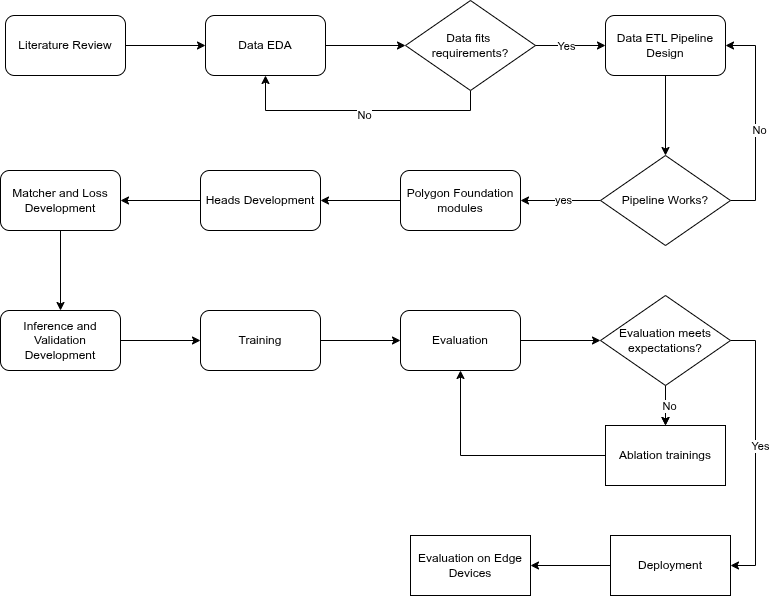
\includegraphics[width=0.55\textwidth]{fig/research-workflow.png}
  \end{center}

\end{frame}

\begin{frame}{Datasets}
  \begin{table}
    \centering
    \begin{tabular}{llll}
      \toprule
      \textbf{Dataset} & \textbf{Purpose} & \textbf{Tissue} & \textbf{Format} \\
      \midrule
      PanNuke & Primary benchmarking & Multi-organ & Pickled bytes \\
      PUMA & TILs detection & Melanoma & TIFF, GeoJSON \\
      panopTILs & TILs detection & Breast & PNG \\
      MoNuSAC & TILs detection & Multi-organ & Pickled bytes \\
      \bottomrule
    \end{tabular}
    \caption{Summary of datasets used in this study.}
  \end{table}

  \begin{itemize}
    \item H\&E stained histopathology images
    \item $\sim$0.25 MPP resolution
    \item Multiple tissue types for generalization
  \end{itemize}
\end{frame}


\begin{frame}{Data Preprocessing Pipeline}
  \begin{center}
    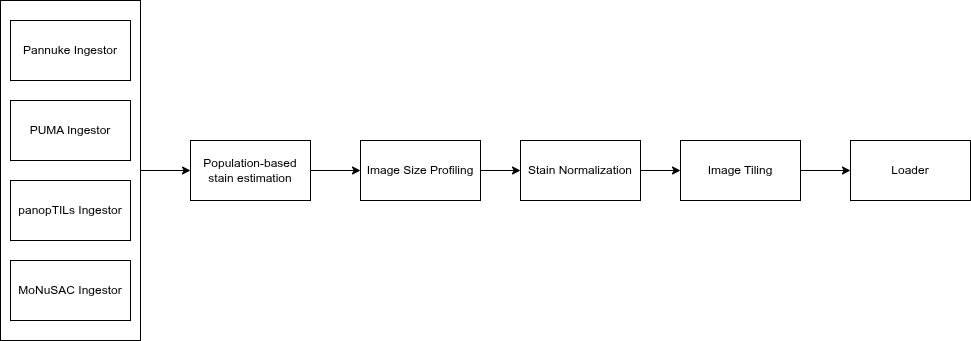
\includegraphics[width=0.9\textwidth]{fig/data-pipeline.png}
  \end{center}
  
  \begin{itemize}
    \item Multi-format dataset handling (TIFF, PNG, pickled bytes)
    \item Patch extraction and augmentation
    \item Star-convex annotation generation
  \end{itemize}
\end{frame}


\begin{frame}{RayCastED Architecture}
  \begin{center}
    \resizebox{0.6\textwidth}{!}{\input{../contents/chapter-3/fig/raycasted.tex}}
  \end{center}

\end{frame}

\begin{frame}{Key Innovations}
  \begin{columns}
    \column{0.5\textwidth}
    \begin{block}{1. RayCast Representation}
      \begin{itemize}
        \item Centroid $(x, y)$ + 12 radial distances
        \item Fixed-angle rays ($0°, 30°, ..., 330°$)
        \item End-to-end differentiable
      \end{itemize}
    \end{block}

    \column{0.5\textwidth}
    \begin{block}{2. End-to-End Assignment}
      \begin{itemize}
        \item Learned bipartite matching
        \item Eliminates NMS dependency
        \item Prevents undercounting in clumps
      \end{itemize}
    \end{block}
  \end{columns}

  \vspace{1em}
  \begin{alertblock}{3. Lightweight FCN Backbone}
    Replaces transformer with YOLO-based FCN for edge deployment (TensorRT/ONNX Runtime)
  \end{alertblock}
\end{frame}



\section{Results}

\begin{frame}{Evaluation Against LSP-DETR}
  \begin{table}
    \centering
    \small
    \begin{tabular}{llll}
      \toprule
      \textbf{Metric} & \textbf{LSP-DETR} & \textbf{RayCastED} & \textbf{Delta} \\
      \midrule
      AJI & \textbf{0.825} & 0.6385 & -0.1865 \\
      FI & \textbf{0.677} & 0.5581 & -0.1189 \\
      mAP@0.5 & \textbf{0.691} & 0.4275 & -0.2635 \\
      Precision & \textbf{0.862} & 0.6848 & -0.1772 \\
      Recall & \textbf{0.791} & 0.5980 & -0.1930 \\
      PQ & \textbf{0.657} & 0.5433 & -0.1137 \\
      SQ & \textbf{0.811} & 0.7460 & -0.0650 \\
      DQ & \textbf{0.810} & 0.6817 & -0.1283 \\
      \midrule
      Params & 45.0M & \textbf{11.92M} & \textbf{-73.5\%} \\
      GFLOPs & - & 4.77 & - \\
      Inference & - & \textbf{4.17ms} & - \\
      \bottomrule
    \end{tabular}
    \caption{Performance comparison with LSP-DETR baseline.}
  \end{table}

    RayCastED achieves \textbf{73.5\% fewer parameters} while maintaining competitive segmentation quality, enabling edge deployment.
\end{frame}


\end{document}
